
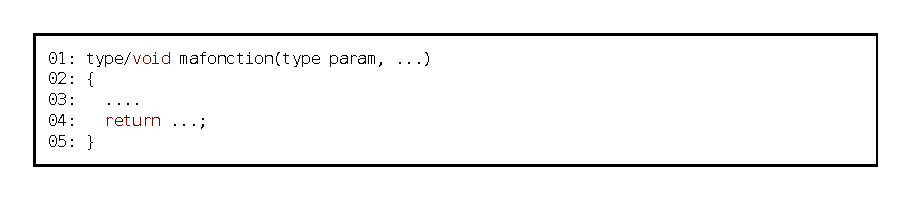
\includegraphics[width=\linewidth]{D8_1.pdf}

\par

\titre{Prototype}
Au début du fichier juste après les instructions pré-processeur \\
Ou dans un fichier header.h

\par

\titre{Portée des variables}
\begin{itemize}
\item Dans une fonction : locale
\item Dans une fonction + static : locale mais la valeur est conservé entre chaque appel
\item En dehors d'une fonction : globale (tout le programme)
\item En dehors d'une fonction + static : tout le fichier
\end{itemize}

\titre{Portée d'une fonction}
\begin{itemize}
\item En général : globale (tout le programme)
\item + static : tout le fichier
\end{itemize} 
